\documentclass[letterpaper,10pt]{article}

\usepackage{titling}
\usepackage{listings}
\usepackage{url}
\usepackage{setspace}
\usepackage{subfig}
\usepackage{sectsty}
\usepackage{pdfpages}
\usepackage{colortbl}
\usepackage{multirow}
\usepackage{multicol}
\usepackage{relsize}
\usepackage{amsmath}
\usepackage{fancyvrb}
\usepackage{amsmath,amssymb,amsthm,graphicx,xspace}
\usepackage[titlenotnumbered,noend,noline]{algorithm2e}
\usepackage[compact]{titlesec}
\usepackage{XCharter}
\usepackage[T1]{fontenc}
\usepackage{tikz}
\usetikzlibrary{arrows,automata,shapes,trees,matrix,chains,scopes,positioning,calc}
\tikzstyle{block} = [rectangle, draw, fill=blue!20, 
    text width=2.5em, text centered, rounded corners, minimum height=2em]
\tikzstyle{bw} = [rectangle, draw, fill=blue!20, 
    text width=4em, text centered, rounded corners, minimum height=2em]

\newcommand{\CPP}{C\nolinebreak\hspace{-.05em}\raisebox{.4ex}{\tiny\bf +}\nolinebreak\hspace{-.10em}\raisebox{.4ex}{\tiny\bf +}}
\def\CPP{{C\nolinebreak[4]\hspace{-.05em}\raisebox{.4ex}{\tiny\bf ++}}}

\let\LaTeXtitle\title
\renewcommand{\title}[1]{\LaTeXtitle{\textsf{#1}}}


\addtolength{\oddsidemargin}{-1.000in}
\addtolength{\evensidemargin}{-0.500in}
\addtolength{\textwidth}{2.0in}
\addtolength{\topmargin}{-1.000in}
\addtolength{\textheight}{1.75in}
\addtolength{\parskip}{\baselineskip}
\setlength{\parindent}{0in}
\renewcommand{\baselinestretch}{1.5}

\singlespace

\begin{document}

\lecture{32 --- Convergence, Ergodicity, Applications}{\term}{Jeff Zarnett}

\section*{Convergence}

Think back to calculus class. Remember when we talk about limits: $\lim_{x\to\infty} f(x)$. There is an answer for this if the function does (somehow) converge on some value, such as the function $f(x) = 1/x^{2}$ converging to 0.

We would like to see that our random variables converge. You might flip a coin four times and all four times it comes up heads. That doesn't match our expectation that we should have about half heads and half tails. We have convergence if, given enough samples and enough sample paths, it will converge to the 0.5 we expect. There may be some sample paths that don't converge (e.g., continually coming up heads), but they have a ``probability mass'' of zero (i.e., they are incredibly unlikely).  There are in fact uncountably many ``bad paths'', each with probability zero (but that's okay). Zero probability doesn't mean it can't happen, mind you.

An image of what convergence looks like~\cite{pmd}:

\begin{center}
	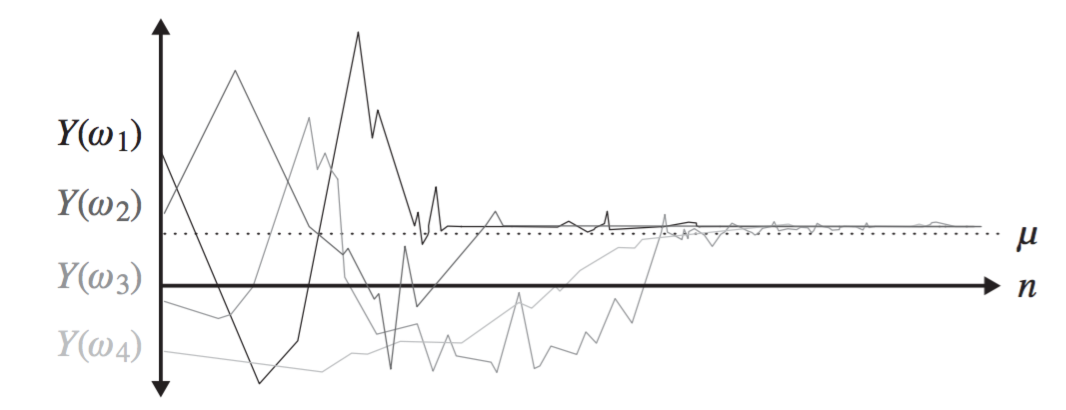
\includegraphics[width=0.6\textwidth]{images/convergence.png}
\end{center}

We won't concern ourselves with systems where there is no convergence. We'll just deal with situations where there is a convergence. Almost every sample path (series of experiments) will eventually behave well if we take enough samples. That is, get past the initial conditions. But sampling is important in our discussion about scalability...

\section*{Tim and Enzo}
A small but important digression on the subject of sampling, measurement, and testing, from~\cite{pmd}. You have an idea of what an average is, but there are two different relevant types of average here---the time average and ensemble average. 

Let us just focus on having a single First-Come-First-Serve queue. Every second, a new job arrives with probability $p$ and if there is any work to do, the job being worked on is completed with probability $q$ (and $q > p$). As a definition, let $N(v)$ equal the number of jobs in the system at a time $v$. In the story, Tim and Enzo are trying to simulate the FCFS system to determine what is the average number of jobs in the system. 

Tim decides he's going to run it as one really long simulation. He simulates the queue over a very long period, logging as he goes, taking a million samples. Then he takes the average value over those samples to get the average number of jobs.

Enzo does something slightly different: instead of having one super long simulation, he does 1000 shorter simulations. He waits until the simulation has run for 1000 seconds and then samples the queue at exactly that point, obtaining one value. This experiment is restarted with a new random seed. So after obtaining a thousand samples, he averages these, and Enzo produces another average number of jobs.

A little illustration of Tim and Enzo from~\cite{pmd}:

\begin{center}
	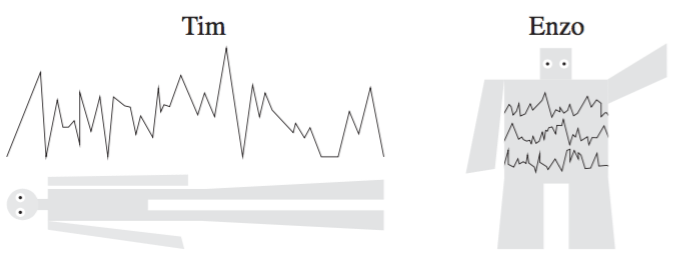
\includegraphics[width=0.5\textwidth]{images/timenzo.png}
\end{center}

So -- who has done this correctly, Tim or Enzo?

The time average has potential problems because we are only looking at a single sequence and maybe something very unusual has happened here in this single run. The ensemble average is more likely what we talk about when we talk about the system being at ``steady state'' (i.e., past the initial conditions). So we kind of like the Enzo approach. Plus, this is programming for performance (or as a student said, programming for parallelism) -- we can do 1000 simulations concurrently if we have enough CPU cores! Tim's approach still has some merit though.

A note about initial conditions: both the Tim and Enzo approaches here require caring about the initial conditions. Enzo needs to make sure that the initial conditions (startup costs etc) have attenuated before the measurement point. Tim needs to ensure that the initial conditions impact a sufficiently small portion of all his measurements.

But! If we have a nicely behaved system, the time average and the ensemble average are the same (so both Tim and Enzo can be correct). What is a nicely behaved system? The word for this is \textit{ergodic}. That probably did not help, so what is an ergodic system? It is a system that is positive recurrent, aperiodic, and irreducible.

\textit{Irreducibility} means a process should be able to get from one state to any other state (where state is the number of jobs in the system). This means the initial state of the system does not matter. So if we started at 0 jobs or 10 we could still get to any state in the system (jobs at 2 or 27)\ldots

\textit{Positive recurrence} means that given an irreducible system, any state $i$ is revisited infinitely often, and the time between visits to that state are finite. So we can define a certain state as being a ``restart''. The logical choice in the case of a queue or similar is the idea of the queue being empty. Every time the queue gets down to zero jobs, it's a ``restart'' of sorts. 

This is what makes Tim's view and Enzo's view potentially the same. A single long run (Tim's view) is just like a number of independent runs (Enzo's view). Every time we get down to zero jobs in the queue, it's a restart. 

The \textit{aperiodicity} condition is required for the ensemble average to make sense or exist. That is to say, the state of the system should not be related to the time; i.e., it is not the case that the system is in state 0 when $t$ is even and state 1 when $t$ is odd. Otherwise the way Enzo chooses to sample, i.e., $t = 1000$, is potentially going to skew the result.

A graphical illustration, also from~\cite{pmd}, that shows how the time average over a single long run can be considered a chain of restarts or ``renewals''.

\begin{center}
	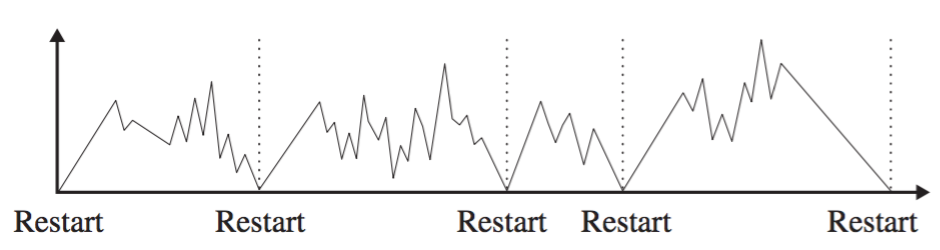
\includegraphics[width=0.5\textwidth]{images/systemrestart.png}
\end{center}

Both Tim and Enzo are correct for ergodic systems. Either method works to determine measurements and queueing theory values. Enzo's method has some advantages, e.g. parallelism and the ability to produce confidence intervals.

We've talked about the average number of jobs, but perhaps what we also care about is how long a job spends in the system, on average. We could compute either the time or ensemble average. 

\begin{center}
	Time Average = $\lim_{t\to\infty}\dfrac{\sum_{i=1}^{A(t)} T_{i}}{A(t)},$
\end{center}

where $A(t)$ is the number of arrivals by time $t$ and $T_{i}$ is the time in the system of arrival $i$. The average is taken over one sample path.

\begin{center}
	Ensemble Average = $\lim_{t\to\infty}E[T_{i}],$
\end{center}

where $E[T_{i}]$ is the average time in the system of job $i$, average being taken over all sample paths.

\section*{Little's Law}
Little's Law is a famous result, saying that the average number of jobs in the system equals the product of the average arrival rate into the system and the average time spent in the system. The source on this section is~\cite{pmd}.

\paragraph{Open Systems.} Let's start with an open system. Here is Little's Law, written more formally:

\[
	E[N] = \lambda E[T],
\]

where $E[N]$ is the expected value of the number of jobs in the system, $\lambda$ is the average arrival rate into the system, and $E[T]$ is the mean time jobs spend in the system. For example, if a University intakes an average of 5,000 students per year and each student spends an average of 4 years in school, then there are $4 \times 5000=20000$ students on average in the University~\cite{sigman-little-law}. The basic setup of Little's Law looks something like this~\cite{pmd}:

\begin{center}
	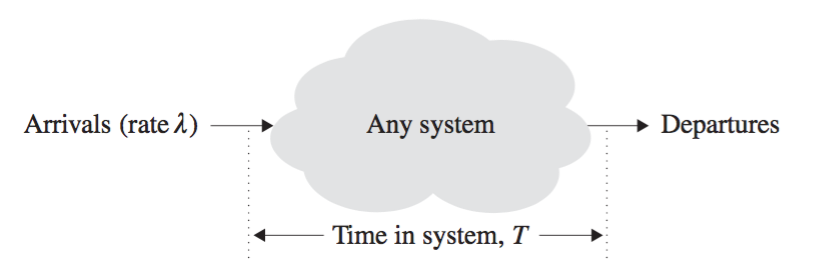
\includegraphics[width=0.5\textwidth]{images/littleslaw.png}
\end{center}

We don't need to know anything about the arrival process (Bernoulli, Poisson, etc\ldots), the service time distribution, network topology, etc. It seems intuitive that this is the case (or it should). Imagine a fast food restaurant: they make money by quick turnaround, so they get people out of the place quickly (low $E[T]$) and accordingly they don't require a lot of seating (low $E[N]$). A sit down restaurant is the opposite though; people leave slowly (high $E[T]$) and therefore the restaurant needs lots of seating (more $E[N]$). This example might seem weird from the perspective of the customer though---from your perspective, you may want to enjoy your evening---but the restaurant is eager to turn your table over, and get you out of there so a new set of guests can be seated. (Another way of looking at this is that restaurants are in the business of renting seats. It's not about food costs.)

If you prefer to think of this in a single FCFS queue version, imagine a customer arrives and sees $E[N]$ jobs ahead of her in the queue. The expected time for each customer to complete is $1/\lambda$, because the average rate of completions is $\lambda $. So we can approximate $E[T]$ as being roughly $\dfrac{1}{\lambda}E[N]$.

\paragraph{Closed Systems.} Remember that for closed systems, we have a rule that says there are $N$ jobs in process at any given time (the multiprocessing level of the system). If the system is ergodic, then $N = X \cdot E[T]$ where $N$ is the multiprogramming level, $X$ is the throughput rate, and $E[T]$ is the mean time jobs spend in the system. This assumes that there is zero think time, i.e., that jobs are always ready at once and don't have to wait for silly users.

If we do have to deal with the vagaries of users and think time, then we care more about the response time $E[R]$. So for a terminal-driven system, the expected response time is $E[R] = \dfrac{N}{X} - E[Z]$ where $N$ is the multiprogramming level, $X$ is the throughput, and $E[Z]$ is the mean time spent thinking. 

\section*{M/M/1}

Probabilistic processes are described according to their models, which will probably be one of the three~\cite{swps}:

\begin{enumerate}
	\item Deterministic (D) -- The process is predictable and characterized by constant factors. For example, the inter arrival times are constant (e.g., a task arrives every minute.)
	\item Markov (M) -- A memoryless process; the future states of the process are independent of the past history. The future state depends on only the present state.
	\item General (G) -- Completely arbitrary.
\end{enumerate}

We're going to focus on Markov processes, because they are nicer (and we have only limited time). It means that the number of arrivals follow the Poisson distribution; the inter-arrival times follow the exponential distribution, and service times follow the exponential distribution too. 

Those letters we saw are part of Kendall notation. It has six symbols, written in a specific order, separated by slashes. The order is $\alpha / \sigma / m / \beta / N / Q$. See the table below for the full explanation:

\begin{center}
\begin{tabular}{l|l} 
	\textbf{Symbol} & \textbf{Meaning} \\ \hline
	$\alpha$ & The type of distribution (Markov, General, Deterministic) \\ \hline
	$\sigma$ & The type of probability distribution for service time \\ \hline
	$m$ & Number of servers \\ \hline
	$\beta$ & Buffer size \\ \hline
	$N$ & Allowed population size (finite or infinite) \\ \hline
	$Q$ & Queueing policy \\ 
\end{tabular}
\end{center}

We often leave off the last three, assuming that there is an infinite buffer, infinite population, and a FIFO queueing policy. If that is the case, then we have only three values. Those three then produce the ``M/M/1'' and ``M/M/k'' symbols. ``M/M/1'' means a Markov arrival process, exponential queueing system, and a single server. When there are $k$ servers, of course the 1 is replaced with the $k$. These are the systems that we are going to examine.

We should also think about utilization, denoted $\rho$. It is a fraction between 0 and 1 and it is simply the amount of time that the server is busy. We talked about this earlier in an informal way, but now we can actually calculate it: $\rho = \lambda \times s$ (the arrival rate and service time). 

For M/M/1 systems, the completion time average $T_{q}$ is $\dfrac{s}{(1-\rho)}$ and the average length of the queue $W$ is $\dfrac{\rho^{2}}{1-\rho}$.

An example from~\cite{williams-q}: we have a server that completes a request, on average, in 10~ms. The time to complete a request is exponentially distributed. Over a period of 30 minutes, 117~000 jobs arrive. So this is a M/M/1 situation. How long did it take to complete the average request? What is the average length of the queue?

The service time $s$ is given as $0.01s$ and the arrival rate is 65 requests per second. So we can calculate $\rho = 0.01 \times 65 = 0.65$. So we have what we need to plug and chug using the formul\ae\ from above to find the time to complete the average request is 28.6~ms and the average length of the queue is 1.21.

What about the number of jobs in the system? The value $\dfrac{\rho^{2}}{1-\rho}$ gives the average number of jobs, including the waiting jobs and the ones being served. It is an average, of course. The probability that there are exactly $x$ jobs in the system at any time is given by the formula: $(1-\rho)\rho^{x}$. The probability that the number of jobs is less than or equal to $n$ is then given by: $\sum\limits_{i=0}^{n}(1-\rho)\rho^{i}$ (the sum of the probabilities of each of the numbers from 0 up to $n$). If you want to know the probability that there are more then $n$ at a time, then you can compute the sum from $n+1$ up to infinity. That might be unpleasant to calculate, but remember that probabilities sum to 1, so you can say that the probability of more than $n$ requests at once is simply $1 - \sum\limits_{i=0}^{n}(1-\rho)\rho^{i}$.

\section*{M/M/k}

Now let us take it to multiple servers ($k$ of them, in fact). We will say jobs arrive at a single queue and then when a server is ready it will take the first job from the front of the queue. The servers are identical and jobs can be served by any server. So far, so simple.

Sadly, the math just got harder. Let's turn again to~\cite{williams-q} as the source for this section. The server utilization for the server farm is now $\rho = \lambda s / N$ (the average utilization for all $N$ servers). To make our calculations a little easier, we want an intermediate value $K$ which looks scary, but is not so bad:

\[ K = \cfrac{\sum_{i=0}^{N-1}\dfrac{(\lambda s)^{i}}{i!}}{{\sum_{i=0}^{N}\dfrac{(\lambda s)^{i}}{i!}}}.
\]

The first term, $i = 0$, is always 1. The denominator is always larger than the numerator, so $K$ is always less than 1. $K$ has no intrinsic meaning, it is just a a computational shorthand so the other formul\ae\  are not so messy.

What is the probability that all servers are busy? We represent this as $C$, the probability a new job will have to wait in the queue.

\[C = \cfrac{1 - K}{1 - \dfrac{\lambda s K}{N}}.\]

The M/M/k formul\ae, then, for the average completion time and average length of the queue are:

\[
  T_{q} = \dfrac{C s}{k(1 - \rho)} + s \mbox{ \qquad\qquad and \qquad\qquad } W = C \dfrac{\rho}{1 - \rho}.
\]

Let's do an example. Suppose we have a printer that can complete an average print job in two minutes. Every 2.5 minutes, a user submits a job to the printer. How long does it take to get the print job on average? We're starting with a single printer, so the system is M/M/1. Service time $s$ is 2 minutes; the arrival rate $\lambda$ is $1/2.5 = 0.4$. So $\rho = \lambda \times s = 0.4 \times 2 = 0.8$. So $T_{q} = s / (1 - \rho ) = 2 / (1 -0.8 ) = 10$. Ten minutes to get the print job. Ouch.

Here we have an opportunity to use the predictive power of queueing theory. Management is convinced that ten minute waits for print jobs is unreasonable, so we have been asked to decide what to do: should we buy a second printer of the same speed, or should we sell the old one and buy a printer that is double the speed?

The faster printer calculation is easy enough. Now $s = 1.0$ and $\lambda$ remains $0.4$, making $\rho = 0.4$. So rerunning the calculation: $T_{q} = s / (1 - \rho ) = 1 / (1 - 0.4 ) = 1.67$. 1:40 is a lot less time than 10:00! 

The two printer solution is more complicated. So let us calculate $K$ as the intermediate value. 

\[K = \cfrac{\sum_{i=0}^{N-1}\dfrac{(\lambda s)^{i}}{i!}}{{\sum_{i=0}^{N}\dfrac{(\lambda s)^{i}}{i!}}} = \cfrac{\dfrac{(\lambda s)^{0}}{0!} + \dfrac{(\lambda s)^{1}}{1!}}{\dfrac{(\lambda s)^{0}}{0!} + \dfrac{(\lambda s)^{1}}{1!} + \dfrac{(\lambda s)^{2}}{2!}} = 0.849057.\]

Now we can calculate $C$ as 0.22857 and $T_{q}$ as 2.38 minutes (by simple plug and chug calculations given the formul\ae\  above). Two observations jump out at us: (1) we doubled the number of printers, but now jobs are completed almost four times faster; and (2) the single fast printer is better, if utilization is low.

That is an important condition: if utilization is low. At some point will the two printers be a better choice than the single fast one? What if both printers are used to the max (100\% load)\ldots?

\section*{Queuing for Performance}

The plan is to take queueing theory and apply it in a performance model. The guide to this section is~\cite{williams-perf}. The basic process is:

\begin{enumerate}[noitemsep]
	\item Convert to common time units.
	\item Calculate the visitation ratios $V_{i}$.
	\item Calculate the device utilization $\rho_{i}$.
	\item Calculate the CPU service time.
	\item Calculate the device time.
	\item Find the bottleneck device.
	\item Calculate the maximum transaction rate.
	\item Calculate the average transaction time.
\end{enumerate}

Let us execute this process on a web server system that serves 9~000 pages per hour. Here are the known values:

\begin{center}
\begin{tabular}{l|r|r|r|r|r|r} 
	\textbf{Device} & \textbf{Data/Hour} & \textbf{$\lambda$} & \textbf{$S$} & \textbf{$V$} & \textbf{$\rho$} & \textbf{$V \times S$} \\ \hline
	Webpages & 9~000 & & & & & \\ \hline
	CPU & & & & &  42\% & \\ \hline
	Disk 1 & 108~000 & & 11ms & & &\\ \hline
	Disk 2 & 72~000 & & 16ms & & &\\ \hline
	Network & 18~000 & & 23ms & & &
\end{tabular}
\end{center}

Step one is to convert to common time units; in this case, seconds. That would be a simple and common time unit. Let's also look at the $\lambda$ values - reported counts divided by seconds in the reporting period.

\begin{center}
\begin{tabular}{l|r|r|r|r|r|r} 
	\textbf{Device} & \textbf{Data/Hour} & \textbf{$\lambda$} & \textbf{$S$} & \textbf{$V$} & \textbf{$\rho$} & \textbf{$V \times S$} \\ \hline
	Webpages & 9~000 & 2.5 & & & & \\ \hline
	CPU & & & & & 42\% & \\ \hline
	Disk 1 & 108~000 & 30 & 0.011s  & & &\\ \hline
	Disk 2 & 72~000 & 20 & 0.016s & & &\\ \hline
	Network & 18~000 & 5 & 0.023s & & &
\end{tabular}
\end{center}

The visitation ratio is the number of times a device is used in each transaction; divide use by number of transactions to get $V_{i}$ (you could also log this sort of thing). The visitation ratio of the CPU is the sum of all other visitation ratios. Why? Suppose we do a disk read: the disk is visited, and when the disk read completes, we go back to the CPU and it picks up the data that's just been shuttled in from the impossibly slow disk.

\begin{center}
\begin{tabular}{l|r|r|r|r|r|r} 
	\textbf{Device} & \textbf{Data/Hour} & \textbf{$\lambda$} & \textbf{$S$} & \textbf{$V$} & \textbf{$\rho$} & \textbf{$V \times S$} \\ \hline
	Webpages & 9~000 & 2.5 & & 1 & & \\ \hline
	CPU & 207~000 & 57.5 &  & 23 & 42\% & \\ \hline
	Disk 1 & 108~000 & 30 & 0.011s  & 12& &\\ \hline
	Disk 2 & 72~000 & 20 & 0.016s & 8 & &\\ \hline
	Network & 18~000 & 5 & 0.023s & 2 & &
\end{tabular}
\end{center}

Next, calculate device utilization: $\rho = \lambda \times s$. That is, arrival rate times service time.

\begin{center}
\begin{tabular}{l|r|r|r|r|r|r} 
	\textbf{Device} & \textbf{Data/Hour} & \textbf{$\lambda$} & \textbf{$S$} & \textbf{$V$} & \textbf{$\rho$} & \textbf{$V \times S$} \\ \hline
	Webpages & 9~000 & 2.5 & & 1 & & \\ \hline
	CPU & 207~000 & 57.5 &  & 23 & 0.42 & \\ \hline
	Disk 1 & 108~000 & 30 & 0.011s  & 12& 0.33 &\\ \hline
	Disk 2 & 72~000 & 20 & 0.016s & 8 & 0.32 &\\ \hline
	Network & 18~000 & 5 & 0.023s & 2 & 0.115 &
\end{tabular}
\end{center}

A small oddity: in the CPU we have a percentage for utilization rather than a decimal number. Just convert it to 0.42. And we can also get the service time of the CPU by rearrangement of the utilization formula to $s = \rho / \lambda$.

\begin{center}
\begin{tabular}{l|r|r|r|r|r|r} 
	\textbf{Device} & \textbf{Data/Hour} & \textbf{$\lambda$} & \textbf{$S$} & \textbf{$V$} & \textbf{$\rho$} & \textbf{$V \times S$} \\ \hline
	Webpages & 9~000 & 2.5 & & 1 & & \\ \hline
	CPU & 207~000 & 57.5 & 0.0073s & 23 & 0.42 & \\ \hline
	Disk 1 & 108~000 & 30 & 0.011s  & 12& 0.33 &\\ \hline
	Disk 2 & 72~000 & 20 & 0.016s & 8 & 0.32 &\\ \hline
	Network & 18~000 & 5 & 0.023s & 2 & 0.115 &
\end{tabular}
\end{center}

And the device time is the final thing we can fill in for this table: $V_{i} \times S_{i}$ (just like the column header says!).

\begin{center}
\begin{tabular}{l|r|r|r|r|r|r}
	\textbf{Device} & \textbf{Data/Hour} & \textbf{$\lambda$} & \textbf{$S$} & \textbf{$V$} & \textbf{$\rho$} & \textbf{$V \times S$} \\ \hline
	Webpages & 9~000 & 2.5 & & 1 & & \\ \hline
	CPU & 207~000 & 57.5 & 0.0073s & 23 & 0.42 & 0.168\\ \hline
	Disk 1 & 108~000 & 30 & 0.011s  & 12& 0.33 & 0.132\\ \hline
	Disk 2 & 72~000 & 20 & 0.016s & 8 & 0.32 & 0.128\\ \hline
	Network & 18~000 & 5 & 0.023s & 2 & 0.115 & 0.046
\end{tabular}
\end{center}

Did we need to complete the whole table? Probably not. In a practical sense what we cared about the most was the $\rho$ column -- utilization. The bottleneck device, i.e., the one that limits our maximum throughput, is the one that is the busiest. Thus, the one with the largest utilization. This application appears to be CPU bound; it has the highest utilization at 42\%, well ahead of disk 1 and disk 2. 

Having identified the bottleneck device as the CPU, we can make a prediction about the maximum rate of transactions (web page requests) we can serve: $\dfrac{1}{S_{i}V_{i}}$ or in this example, 5.95. This is also called saturation. If $\lambda$ exceeds this saturation point, we will not be able to keep up with incoming requests.

With this table we can also calculate the average transaction time: it is the sum of the $S_{i}V_{i}$ columns. In this example, it is 0.474 seconds. 

\paragraph*{It Gets Worse}

The typical assumption is that we know the service times for each device. Unfortunately this is not true; usually performance monitoring gives us the average size of a device queue. So we had better apply queuing theory here, once again credit to~\cite{williams-calc} for the section. 

The average size of a device's queue is $W$, and for a queue with characteristics M/M/1 then $W = \dfrac{\rho^{2}}{1-\rho}$. Combining the known $W$ with the average arrival rate $\lambda$, we can work out the service time. $W = \dfrac{(\lambda s)^{2}}{1 - \lambda s}$, so:

\[ s = \cfrac{-w \pm \sqrt{w^{2}+4w}}{2\lambda}.\]

Yup. The quadratic formula strikes back. 


\bibliographystyle{alphaurl}
\bibliography{459}


\end{document}
